%!TEX root = paper.tex
%%%%%%%%%%%%%%%%%%%%%%%%%%%%%%%%%%%%%%%%%%%%%%%%%%%%%%%%%%%%%%%%%%%%%%%%%%%%%%%%
\section{Overview and Background}
\label{sec:background}

Before diving into the promised end-to-end lag model, some terms and concepts need to be introduced first.


\subsection{Some Video Game Flavors}
%TODO: needs a better word than types, more like architectures. Feedback welcome

\begin{figure}[!t]
\centering
\removelatexerror
\begin{algorithm}[H]
 \While{game running}{
  read inputs\;
  update game state\;
  render screen\;
 }
\end{algorithm}
\caption{Basic model of a continuous main video game loop.}
\label{alg:gameloop1}
\end{figure}

At their core video games are essentially feedback-directed real-time simulators. The simplified simulator's main loop consists of three central parts as depicted in Fig.~\ref{alg:gameloop1}. Every render-call means putting out a new video frame. As this \textbf{framerate} is usually not limited and variable, the game logic has to update its state on a time-scale operating independent of the current frame. Some games also update parts of the game on one or mulitple fixed frequencies, the so-called \textbf{tickrate}, for example a non-game-influencing physics effect could be updated at a lower \SI{30}{\hertz} rate. The components of a locally running \textit{singleplayer game} and their interactions are depicted in Fig.~\ref{fig:component-model-local}.

\begin{figure}
  \centering
  \includegraphics[width=0.8\columnwidth]{../models/component_interaction-local.pdf}
  \caption{Components and interactions of a singleplayer video game.}
  \label{fig:component-model-local}
\end{figure}

\begin{figure}
  \centering
  \includegraphics[width=0.8\columnwidth]{../models/component_interaction-online.pdf}
  \caption{Components and interactions of an online video game. Local game state is synchronized with the server's view on the game state.}
  \label{fig:component-model-online}
\end{figure}

\textit{Online video games} (i.e. mostly multiplayer games) complicate this update logic a bit as seen in the depiction of Fig~\ref{fig:component-model-online}. In client/server online games, the client is not the final authority over its game state any more. Instead, interpreted input commands are sent to the server and a preliminary game state is calculated locally. When the authoritative update from the server is received the two states can be once again be synchronized. 
A third typical component of online video games is the \textbf{command message rate}, i.e., the rate at which input is sent from the client to the server as well as game state updates from the server to the clients do not need to be the same rate as the server's tick rate. Popular examples for the fixed tickrates of game servers include \SI{64}{\hertz} or \SI{128}{\hertz} for \textsc{Counter-Strike: Global Offensive}, \SI{20}{\hertz} for \textsc{Minecraft}, or \SI{30}{\hertz} for \textsc{Dota 2}.

\begin{figure}
  \centering
  \includegraphics[width=0.8\columnwidth]{../models/component_interaction-cloud.pdf}
  \caption{Components and interactions of a streamed video game. I/O and game engine are physically separated and have to be synchronized.}
  \label{fig:component-model-cloud}
\end{figure}


The crucial components of \textit{cloud gaming} are not much different than local or online video games as shown in Fig~\ref{fig:component-model-cloud}. Generally speaking, cloud gaming is a form of \textit{game streaming} where the game streaming server is part of a larger streaming service and hosted at a data center. Through the spatial separation of the input/output devices and the game engine, input data needs to be send from the client to the server and the processed video data is transmitted back to the client in a lossy encoded form.

\begin{figure}[!t]
	\centering
	\includegraphics[width=1.0\columnwidth]{../models/game-tick-rate-streamed.pdf}
	\caption{Interaction of client and server in streamed online games.}
\label{fig:tickrate-streamed}
\end{figure}

Fig.~\ref{fig:tickrate-streamed} gives once again an overview of all these components for a combined streamed online video game scenario.


%%%%%%%%%%%%%%%%%%%%%%%%%%%%%%%%%%%%%%%%%%%%%%%%%%%%%%%%%%%%%%%%%%%%%%%%%%%%%%%%
\subsection{Framerate and Frame-times}
\label{sec:framerate}

In contrast to traditional video media with their fixed framerates of, e.g., \SI{24}{\hertz} or \SI{29.97}{\hertz}, video games are more flexible but simultaneously also much more demanding to the framerate for several reasons. First, video games usually target frame rates of \SI{30}{\hertz}, \SI{60}{\hertz}, or sometimes also \SI{120}{\hertz}, depending on the type of game. Higher frame rates are targeted to enable smoother camera movement and scene transitions, as games often present faster scenes when compared to videos. High frame rates also help in increasing the interactivity as video games constantly require input on short time scales to which the game reacts and displays the feedback. Therefore, the framerate also influences the reactivity of a game and can also be a source of latency itself.

%Generally speaking, motion in video data is based on the principle of \textit{apparent motion}. In order to perceive objects to be in motion in videos, consecutive images have to appear at a certain rate which is considered to be at about \SI{16.67}{\hertz} according to \cite{wertheimer1912experimentelle}. Below that threshold objects will appear as two distinct objects between two consecutive frames. %This form of apparent movement is called the phi phenomenon. The higher the rate of displaying images, the more fluid the motion looks, as the discrete ``jumps'' in the position of the object get smaller the higher the framerate is.\footnote{One can verify this behavior for example at \url{https://frames-per-second.appspot.com/}.}.

% In general, there is no commonly established upper limit to the framerate that humans can still perceive as an improvement to motion presentation, the gain has however diminishing returns. The typical movie framerate of \SI{24}{\hertz} is considered to be at the lower end of motion perception but mostly still works without any problem due to the presence of motion blur. This artifact is always present in recorded images as objects are still in motion during film exposure. %A faster shutter speed reduces the amount of motion blur. % film grain also has an influence

% \begin{figure}[!t]
% 	\centering
% 	\includegraphics[width=1.0\columnwidth]{images/framerate.pdf}
% 	\caption{Effects of frame rate and motion blur on the smoothness of movement and spatial resolution. Objects move at the same speed to the right only the position os updated at different rates. A depiction of strong motion blur was added to the right-hand side.}
% \label{fig:framerate}
% \end{figure}

% The benefit of motion blur lies in its ability to conceal stutters in apparent movement due to the object and its edges being blurred, thereby reducing the positional information available on it.%, Figure~\ref{fig:framerate} illustrates this. 
% Therefore, typical movie sequences usually appear to be perfectly fluid. Only for example when the camera pans at a high speed stutters in object movement or the viewport updates become apparent. Intrinsic motion blur is absent in computer generated imagery but can be artificially added to the images. While adding blur to video games can improve fluidity, it also reduces the spatial information available to the player and hampers the precision of the player's actions. Therefore it is often avoided, especially for objects in focus.

% Video games add two more factors to the frame rate consideration. The first is the issue of the monitor's refresh rate. Monitors work with a fixed, configurable image refresh rate, typically always including \SI{60}{\hertz}. If the game outputs images at an inconsistent rate or a rate lower than the monitor's refresh rate or if the framerate is not an integer multiple of the refresh rate or vice versa one of two things will happen: tearing or stuttering. % TODO: shorten and rephrase this section

% \begin{itemize}
% 	\item If the monitor fetches a frame from the graphics card's buffer while the frame is still being rendered, the result will be a mixture of the new frame in the upper half of the image and a frame which is one time interval older. This artifact is called \textbf{tearing} and should be avoided.
% 	% only the upper portion of the frame  finished, One frame split up between two refresh cycles
% 	\item Games can also be configured to postpone the rendering of a new frame until the monitor has already fetched and displayed the current frame, this is called waiting for vertical synchronization or \textbf{VSYNC}. No tearing will occur, but the \gls{IAT} of new frames might become very irregular, displaying some frames more often than others just to match the monitors refresh rate, resulting in a stuttering display. This latter stuttering effect also occurs for \SI{24}{\hertz} movies being displayed on a \SI{60}{\hertz} TV screen. Therefore most TVs additionally provide a dedicated \SI{24}{\hertz} refresh rate mode to remove the stuttering.
% \end{itemize}




%%%%%%%%%%%%%%%%%%%%%%%%%%%%%%%%%%%%%%%%%%%%%%%%%%%%%%%%%%%%%%%%%%%%%%%%%%%%%%%%
\subsection{End-to-End Lag}

Traditionally, lag in video gaming has often been described as solely the network delay in an online game, which is often also called the ``ping''. It should be evident that the lag is a critically important factor for almost all games, but espiaclly for fast games or competitive games, as it governs the reaction time to in-game events.

But this focus on network delay neglects some key components to this lag, including the input device, the time to sample and process the input, the game engine and server and their tickrates, frame rendering time, and ultimately the time to display the frame on the monitor. Only if all sources are factored in the complete \textbf{end-to-end lag} is captured. What makes matters even worse, is that this lag is usually not constant but can vary depending on the type of action triggered by the input. While some simple actions, say opening the menu, may have a very short lag, more complex interactions, e.g., issuing a move command, may take considerable longer to complete especially when the game is not performing well, partly due to the actions taking more than one game tick to complete. Therefore, each video game will have a distinct ``lag profile''.  


TODO:
This subsection adds the player to the architectures introduced above, highlights potential QoS and QoE (or discusses why some chosing a particular QoE metric is not useful) metrics to study. At the end of this section, the reader should agree that end to end latency is a sensible starting point to study video game qos.


%%%%%%%%%%%%%%%%%%%%%%%%%%%%%%%%%%%%%%%%%%%%%%%%%%%%%%%%%%%%%%%%%%%%%%%%%%%%%%%%
\subsection{Measurement Approaches}
\label{sec:measurementapproaches}

With the central role of the end-to-end lag in mind, it is natural to assume, that this lag should also play a critical role in both subjective and objective video game quality assessments. Therefore, the end-to-end lag needs to be correctly measuremed and determined correctly from any kind of video game. But video games usually represent a black box with very few points, where something can be actually measured. The following sections discuss three distinct methods which are each situated at a unique vantage point as depicted in Fig.~\ref{fig:measurement-methods}.

\begin{figure}[!t]
    \centering
    \includegraphics[width=1.0\columnwidth]{../models/e2e-lag.pdf}
    \caption{Location of the three measurement approaches to capture end-to-end latency inside a usual online video game lag chain.}
\label{fig:measurement-methods}
\end{figure}

%%%%%%%%%%%%%%%%%%%%%%%%%%%%%%%%%%%%%%%%%%%%%%%%%%%%%%%%%%%%%%%%%%%%%%%%%%%%%%%%
\paragraph{Screen Recording Software Method}
Recording the output stream of a video game might be the simplest approach to determine video game lag. It can capture both the framerate and \gls{IAT} at a driver level, and the recorded video can be used for image and quality analyses as well as to correlate it to additionally recorded input events in order to calculate the lag. This is not the complete end-to-end lag however, as both the controller and screen output latency are missing. The need to install additional software might make it unsuitable for some scenarios, e.g., when measuring console video games. As a variant of this method, one can also record the output stream with a video capture card on a secondary computer, which does not negatively effect the game's performance as the software method would.

Examples of this approach include both \cite{Chen:2011:MLC:2072298.2071991} and \cite{6670099} which measured the latency of cloud gaming services in the game client. They do this by invoking the system menu in games and measuring the time until it is displayed. A 2013 paper \cite{6574660} investigates the quality of cloud gaming interactiveness (i.e., the lag) as well as image quality by employing software recording methods on the client's computer.
%However, this method assumes a constant delay of game actions and may not capture the actual end-to-end lag of many of real game actions, as they are typically different from and longer as the latency of displaying a menu. A 2013 paper \cite{6574660} investigates the quality of cloud gaming interactiveness (latency) as well as image quality by employing software recording methods on the client's computer. With these techniques the challenges regarding the quality are discussed.


%%%%%%%%%%%%%%%%%%%%%%%%%%%%%%%%%%%%%%%%%%%%%%%%%%%%%%%%%%%%%%%%%%%%%%%%%%%%%%%%
\paragraph{Passive Network Measurements}
In some cases it may also be advantageous to tap into the network interactions of the games and record the command and update messages sent between server and clients. While this is not a direct measure of game quality, it can give insights into the game's inner workings, such as the tick rates, and one can derive, e.g., the lowest achievable end-to-end lag from this.

%Can only investigate command and update messages, not tick rate directly. Evaluate rate, IAT, and bandwidth, estimate latency (though there may be no direct link between commands and updates).

% Besides simple flow-based or packet-counting network metrics, many games also allow for deeper packet-dissecting analyses, as the often rely on standardized protocols or data formats, such as Protobuf\footnote{\url{https://developers.google.com/protocol-buffers/}} or incorporate well-known third-party multiplayer-enabling libraries. %And cloud games sometimes use derivates from the RTP-family or XMPP-based(VERIFY) protocols. 
% Additionally, almost no game encrypts its time-critical messages, enabling an easy read-out. Through these means, the specific commands can be read from the network and potentially linked to their effect on the game state in the corresponding state update messages.
%, but also potentially allowing malicious actions to be taken easily.


%%%%%%%%%%%%%%%%%%%%%%%%%%%%%%%%%%%%%%%%%%%%%%%%%%%%%%%%%%%%%%%%%%%%%%%%%%%%%%%%
\paragraph{Camera Recordings}
Finally, the only method to fully capture the end-to-end lag is to simultaneously record both the screen and input device through an external camera. The experimenter then has to count the frames between pressing a button on the input device and the action appearing on the screen and calculate the lag from this. For better visibility the input device is usually modified with an LED that turns on when the button is pressed. Also, the camera should operate at least at twice the monitor's refresh rate according to the Nyquist-Shannon sampling theorem. An additional benefit of this method is, that the game and the computers remain unaltered and are therefore not affecting any properties of the game. A variant of this approach, replacing the camera with a photodiode and synthetically creating the input events with a microcontroller is described in \cite{beyermethod}, though it may be difficult to use for certain game actions that have a barely visible or unpredictable on-screen effect.




% \begin{figure}
%   \centering
%   \includegraphics[width=0.8\columnwidth]{../models/component_interaction-online+cloud.pdf}
%   \caption{Interaction of TODO.}
%   \label{fig:component-model-online+cloud}
% \end{figure}

% \begin{figure}
%   \centering
%   \includegraphics[width=1.0\columnwidth]{../models/cycle.pdf}
%   \caption{Interaction of TODO.}
%   \label{fig:component-model}
% \end{figure}